\documentclass[journal]{IEEEtran}
\usepackage{amsmath,amssymb}
\usepackage{booktabs}
\usepackage{graphicx}
\usepackage{adjustbox}
\usepackage{url}
\usepackage{cite}
\hyphenation{Retrieval-Augmented}

\begin{document}

\title{Bridge Failure in Retrieval-Augmented Generation: Measuring It and Repairing It with Connectivity-Aware Context Selection}

\author{Pavan~Kumar~Mantha,
        Nenavath~Srinivas~Naik,
        and~Naresh~Babu~Muppalaneni%
\thanks{P. K. Mantha, N. S. Naik and N. B. Muppalaneni: [affiliation to be completed by the authors].}}

\markboth{Manuscript draft}{Mantha \MakeLowercase{\textit{et al.}}: Bridge Failure in RAG}
\maketitle

\begin{abstract}
Multi-hop questions often fail in retrieval-augmented generation (RAG) because the context contains the endpoints of a reasoning chain but not the bridge passage that links them. We call this \emph{bridge failure} and measure its cost: across four generators from two vendors, answer F1 is 72.6--79.9\% when the context contains all gold passages and 19.2--24.1\% when it does not, and the generators abstain on 53--63\% of bridge-failed contexts. We propose SES-RAG, a greedy context selector that makes no LLM call and adds to each candidate's relevance the change in the algebraic connectivity (Fiedler value) of the selected evidence subgraph under a token budget. On 861 HotpotQA bridge questions that were not used for tuning, it retrieves a complete context about 10 points more often than Hybrid RAG and improves F1 by 4.0--6.5 points for every generator; on 2WikiMultiHopQA it improves gold-complete retrieval by 8--19 points over all LLM-free baselines without re-tuning. The evidence also sets clear limits. SES-RAG is not significantly better than the strongest graph baselines on HotpotQA, ties them on MuSiQue, and trails an LLM-driven iterative retriever by 11 points of gold-complete retrieval and 7--10 points of F1 on HotpotQA (22 points of gold-complete retrieval on 2WikiMultiHopQA). Simpler connectivity rewards (component count, unnormalised $\lambda_2$) are statistically indistinguishable from the spectral one after multiple-comparison correction, its advantage over the same selector without the connectivity term disappears when the graph lacks title-mention edges, and combining iterative retrieval with the same packing rule gives no significant gain on HotpotQA and a loss on MuSiQue. We release code, frozen parameters and all model outputs.

\end{abstract}

\begin{IEEEkeywords}
retrieval-augmented generation, multi-hop question answering, context selection, graph connectivity, spectral graph theory
\end{IEEEkeywords}

\section{Introduction}
\label{sec:intro}

Retrieval-augmented generation (RAG)~\cite{lewis2020rag} grounds a language model in retrieved passages, but many questions cannot be answered from any single passage. In \emph{bridge} questions~\cite{yang2018hotpotqa} the second passage is reachable only through an entity named in the first, and the question itself never mentions that entity: ``Which university did the director of \emph{Film X} attend?'' needs the passage about the film, which names the director, \emph{and} the passage about the director. Similarity-based retrieval ranks the second passage low because it shares little vocabulary with the question. The generator then sees the endpoints of the reasoning chain without the link between them and either abstains or guesses. We call this \emph{bridge failure}.

Remedies fall into two families. \emph{Iterative retrieval} lets an LLM reformulate the query after each round~\cite{trivedi2023ircot,asai2024selfrag}; it works but costs several LLM calls per question. \emph{Graph-based RAG} builds entity or passage graphs and uses them to find or re-rank candidates~\cite{edge2024graphrag,guo2024lightrag,gutierrez2025hipporag2,he2024gretriever,rappazzo2024gem}; the graph typically scores passages \emph{one at a time}. Neither family reasons directly about the property that matters for a bridge question: whether the \emph{set} of passages that will be shown to the generator is connected through the bridge.

We ask four questions. \textbf{RQ1:} how much of the answer-quality loss on bridge questions is attributable to a bridge-failed context, as opposed to generator behaviour? \textbf{RQ2:} can a cheap selector that uses no LLM call, and rewards a \emph{connected} context under a token budget, repair bridge failure better than flat retrieval and graph-based baselines? \textbf{RQ3:} is spectral connectivity (the Fiedler value $\lambda_2$ of the selected subgraph) the active ingredient, or would any connectivity reward do? \textbf{RQ4:} when does the effect transfer across graphs, generators and datasets?

We propose SES-RAG (Spectral Evidence Selection RAG), a greedy context selector that adds to the relevance of each candidate the change in $\lambda_2$ of the induced evidence subgraph, and evaluate it against seven baselines, a gold-first oracle and four generators from two vendors, under a protocol with a held-out primary set, equal tuning effort, Holm-corrected paired tests and a pre-declared pass criterion. Our contributions are:
\begin{itemize}
\item \textbf{A measurement of bridge failure} (RQ1). Conditioning on whether the context contains all gold passages separates retrieval from generation: with a complete context the four generators reach 72.6--79.9\% F1, with a bridge-failed one 19.2--24.1\%, and they abstain on 53--63\% of failed contexts.
\item \textbf{SES-RAG}, a set-level, LLM-free selector (RQ2). It is the best method that makes no LLM call on HotpotQA bridge questions, improving gold-complete retrieval by about 10 points over Hybrid RAG and F1 by 4.0--6.5 points, with confidence intervals excluding zero for all four generators. It does not significantly beat the strongest graph baselines, and an LLM-driven iterative baseline is ahead of it.
\item \textbf{Negative and boundary results} (RQ3, RQ4). Component count and raw-$\lambda_2$ connectivity terms work as well as or better than normalised $\lambda_2$, so spectral connectivity is not special; the advantage appears on 2WikiMultiHopQA but not on MuSiQue, disappears when the graph lacks title-mention edges, and an extension that packs iterative-retrieval candidates with the same rule gives no significant gain on the primary set.
\item \textbf{A pre-specified, reproducible evaluation protocol} with a held-out primary set, equal tuning effort per system, frozen parameters, and code and raw outputs released.
\end{itemize}

\section{Related Work}
\label{sec:related}

\paragraph{Multi-hop question answering and iterative retrieval.}
HotpotQA~\cite{yang2018hotpotqa}, 2WikiMultiHopQA~\cite{ho2020constructing} and MuSiQue~\cite{trivedi2022musique} require combining several documents, and in \emph{bridge} questions the second document is reachable only through an entity named in the first. Single-shot dense retrieval~\cite{karpukhin2020dpr,lewis2020rag} ranks the second document low because the question never mentions its entity. The standard remedy is iterative retrieval: IRCoT~\cite{trivedi2023ircot} interleaves retrieval with chain-of-thought steps, and critique-based approaches such as Self-RAG~\cite{asai2024selfrag} decide when and what to retrieve again. These methods issue several LLM calls per query. We include an iterative baseline and show how it compares with an LLM-free alternative.

\paragraph{Graph-based RAG.}
GraphRAG~\cite{edge2024graphrag} and LightRAG~\cite{guo2024lightrag} build entity graphs with an LLM and retrieve through entities and community summaries; HippoRAG~\cite{gutierrez2024hipporag} and HippoRAG~2~\cite{gutierrez2025hipporag2} run Personalized PageRank~\cite{haveliwala2002ppr} over an entity--passage graph; G-Retriever~\cite{he2024gretriever} selects a connected subgraph by solving a prize-collecting Steiner tree problem. GEM-RAG~\cite{rappazzo2024gem} and SpectRAG~\cite{spectrag} use the eigenvectors of a normalised graph Laplacian as chunk coordinates for proximity scoring. In all of these, the graph generates or re-ranks \emph{individual} candidates. We instead score the \emph{set} that will be shown to the generator.

\paragraph{Budgeted context selection.}
AdaGReS~\cite{peng2025adagres} greedily selects chunks under a token budget with a set-level relevance and redundancy objective; SEAL-RAG~\cite{lahmy2025seal} replaces distractors with missing bridge facts under a fixed retrieval depth; PAGE-RAG~\cite{deng2026page} uses a graph as a query-aware filter over a candidate pool under a fixed budget. PAGE-RAG and SEAL-RAG are the closest in motivation. Our selector differs in its objective: it adds the change in the algebraic connectivity of the selected subgraph to the relevance gain and needs no LLM call. Ex-GraphRAG~\cite{sade2026exgraphrag} studies which retrieved subgraph evidence reaches a GNN-based generator, which is complementary.

\paragraph{Spectral graph theory.}
The second-smallest eigenvalue $\lambda_2$ of a graph Laplacian, the Fiedler value~\cite{fiedler1973algebraic,chung1997spectral}, is zero if and only if the graph is disconnected and grows with connectivity; its eigenvector underlies spectral partitioning~\cite{shi2000normalized}. We use $\lambda_2$ of the subgraph induced by the \emph{selected context} as a connectivity signal.

\paragraph{Positioning.}
Prior work establishes that bridge evidence matters and that graphs can help find it. What is missing is (i) a measurement of how much of the answer-quality loss on bridge questions is attributable to a missing bridge paragraph, separately from generator behaviour; (ii) a comparison of a cheap, LLM-free, set-level connectivity selector against flat, graph-based and LLM-iterative baselines under the same chunks, graph, budget and generators; and (iii) an ablation of whether spectral connectivity specifically, as opposed to any connectivity bonus, is responsible for the gain. This paper supplies these.

\section{Problem and Method}
\label{sec:method}

\subsection{Bridge-complete contexts}
Let $\mathcal{C}$ be a corpus of chunks (here one chunk is one paragraph, and we use ``chunk'', ``paragraph'' and ``passage'' interchangeably) and $q$ a question. A generator receives a context $S\subseteq\mathcal{C}$ with token cost $\tau(S)=\sum_{c\in S}\tau(c)\le B$. For a bridge question, let $G_q\subseteq\mathcal{C}$ be the gold supporting chunks (two or more, linked by a bridge entity). We call $S$ \emph{bridge-complete} (``gold-complete'' in the tables) if $G_q\subseteq S$ and \emph{bridge-failed} otherwise; bridge-failed thus covers any missing gold chunk, in practice usually the bridge chunk. Since the bridge chunk has low lexical and semantic similarity to $q$, similarity-ranked contexts are bridge-failed more often than their per-chunk recall suggests. Our measurements (Section~\ref{sec:results}) quantify the effect on answer quality by conditioning on completeness.

\subsection{Evidence graph}
We build one undirected weighted graph $G=(\mathcal{C},W)$ over the corpus, shared by every graph-based method. Three edge signals are combined,
\begin{equation}
W_{ij}=0.5\,m_{ij}+0.2\,\min\!\left(1,\tfrac{s_{ij}}{3}\right)+0.3\,\kappa_{ij},
\end{equation}
where $m_{ij}=1$ if the text of one chunk mentions the title of the other, $s_{ij}$ is the number of shared capitalised entity spans (spans occurring in more than 20 chunks are ignored), and $\kappa_{ij}\in[0,1]$ is the min--max normalised cosine similarity for the six nearest neighbours of each chunk. Edges with $W_{ij}<0.1$ are dropped. The title-mention signal plays the role of hyperlinks between encyclopedia articles; Section~\ref{sec:results} reports what happens without it.

\subsection{Candidate pool and relevance}
For each query we compute dense (cosine) and BM25~\cite{robertson2009bm25} scores, fuse the two rankings with reciprocal rank fusion~\cite{cormack2009rrf}, and take the top ten as seeds. The pool consists of the seeds plus their graph neighbours up to two hops (at most 8 and 5 strongest neighbours per node at hops one and two), capped at 100 chunks. Relevance is $r(c)=0.7\,\min\!\big(1,\max(0,\tfrac{\cos(q,c)-\bar{\cos}}{\max\cos-\bar{\cos}})\big)+0.3\,\tfrac{\mathrm{bm25}(q,c)}{\max\mathrm{bm25}}$ with the mean and maximum taken over the corpus, and is min--max normalised within the pool before selection. The IRCoT+SES pool is the union of this pool and the iterative hits and may exceed 100 chunks. SpectRAG-lite uses the top five seeds.

\subsection{SES-RAG selection}
For a set $S$ let $G[S]$ be the subgraph induced by $S$ and $L_S=I-D^{-1/2}W_SD^{-1/2}$ its normalised Laplacian, where the rows and columns of zero-degree nodes are set to zero. Let $\lambda_2(S)$ be its second-smallest eigenvalue, with the convention $\lambda_2(S)=0$ for $|S|\le 1$; for $|S|\ge 2$, $\lambda_2(S)=0$ exactly when $G[S]$ is disconnected. SES-RAG greedily builds $S$ under the token budget:
\begin{equation}
c^\star=\arg\max_{c\notin S,\;\tau(S\cup c)\le B}\; r(c)+\mu\big(\lambda_2(S\cup\{c\})-\lambda_2(S)\big).
\label{eq:ses}
\end{equation}
Three properties of the normalised $\lambda_2$ shape the behaviour of this rule. (i) For two nodes joined by any edge $\lambda_2=2$ whatever the edge weight, so the first connected step jumps from $0$ to $2$ and the weights of Eq.~(1) matter only for larger sets. (ii) Adding a node to a connected set usually \emph{lowers} $\lambda_2$ (for unit-weight paths of $2$, $3$ and $4$ nodes it is $2$, $1$ and $0.5$), whereas adding a node that is not connected to the set drops it to $0$. The term therefore penalises fragmenting the selection more than it penalises growing a connected chain, and it rewards the first link most. (iii) If $S$ already has several components, a chunk that joins only two of them earns no reward. The greedy rule has no submodularity guarantee; the term is a connectivity heuristic, not an optimal-evidence criterion. Each step evaluates at most $|{\rm pool}|=100$ eigenvalue problems on matrices of size at most $|S|+1$, which takes milliseconds on a CPU and requires no LLM call. With $\mu=0$ the method reduces to relevance-ranked selection from the graph-expanded pool (the ``Hybrid+Expand'' control).

\subsection{Extension: iterative retrieval with connectivity-aware packing}
IRCoT-style retrieval produces strong candidates but fills the budget in retrieval order. We add the chunks retrieved over $R$ iterative rounds to the pool, give them a relevance bonus $\beta$, and apply the same greedy rule~(\ref{eq:ses}). We call this system IRCoT+SES. Its parameters $(\mu,\beta)$ were selected on the development and exploration questions only.

\section{Experimental Setup}
\label{sec:setup}

\paragraph{Datasets and corpus protocol.}
We sample 2{,}000 questions from the HotpotQA distractor validation set (seed 42) and pool all of their paragraphs into one corpus of 19{,}264 paragraphs, so retrieval must discriminate against distractors from other questions. 1{,}604 of the questions are of the bridge type. Questions are split into a development set (243 bridge questions), an exploration set (the first 500 test bridge questions), and a \emph{primary evaluation set} of 861 test bridge questions that is never used for tuning. As external datasets we use 1{,}000 answerable MuSiQue validation questions (11{,}515 paragraphs) and 1{,}000 compositional and inference questions from 2WikiMultiHopQA (5{,}173 paragraphs), each evaluated on 500 test questions with the settings frozen on HotpotQA. Comparison-type questions are outside the scope of this study.

\paragraph{Protocol and disclosures.}
The bridge-only scope was chosen after an earlier mixed-type run in which the connectivity reward hurt comparison questions. Of the 861 primary questions, 500 had already been used in a first exploratory evaluation with a local generator (never for tuning), and 361 were untouched. Parameters were tuned on the development and exploration questions only. The parameters of IRCoT-lite and IRCoT+SES were added to the frozen file after the other systems' primary-set retrieval had been computed, again using only development and exploration questions. The budget and $\mu$ sweeps and the error analysis were run on the primary set afterwards and are exploratory. Each parametrised system had a grid of four or five settings; pool size, graph weights and relevance mixing were fixed by hand for all graph-based systems and not tuned.

\paragraph{Baselines.}
All systems use the same chunks (one paragraph each), embedder (text-embedding-3-small), candidate machinery and 600-token budget. \textbf{Naive RAG}: dense top-$k$. \textbf{Hybrid RAG}: dense and BM25 fused by RRF. \textbf{Hybrid+Expand} ($\mu{=}0$): SES-RAG without the connectivity term. \textbf{GraphRAG-lite}: entity-linked local search (query entities matched to chunk titles and mentions, expanded one hop). \textbf{SpectRAG-lite}: relevance mixed with spectral-coordinate and Personalized PageRank proximity to the seeds. \textbf{G-Retriever-lite}: a Steiner-tree connection of the top-ranked chunks, filled by relevance. \textbf{IRCoT-lite}: three rounds in which an LLM (gpt-4o-mini) writes a follow-up search query from the evidence so far. A \textbf{gold-first oracle} is reported as a ceiling only. The ``-lite'' systems are our re-implementations of the retrieval principle of each method on the shared graph, not the original systems; they omit LLM-built graphs, community summaries and learned components. Each parametrised system was tuned with a grid of four or five settings on the development and exploration questions (retrieval completeness as criterion) and then frozen: SES-RAG $\mu{=}0.25$, SpectRAG-lite mixing weight $0.25$, G-Retriever-lite four terminals, GraphRAG-lite bonus scale $0.25$, IRCoT-lite three rounds of two chunks, IRCoT+SES $\mu{=}0.5$, $\beta{=}0.5$.

\paragraph{Generators and judging.}
Answers are produced with four generators from two vendors: gpt-4o-mini (primary), gpt-4o~\cite{hurst2024gpt4o}, claude-sonnet-5-5 and claude-haiku-5-5~\cite{anthropic2026claude}; embeddings use text-embedding-3-small~\cite{openai2024embed}. Context chunks are shown in a per-question random order~\cite{liu2024lost} so no system benefits from ordering. The prompt asks for a short answer using only the context, or INSUFFICIENT. OpenAI models use temperature 0; the Claude models used here accept no temperature parameter and run with default sampling, with extended thinking disabled (claude-haiku-5-5) or restricted to between tool calls (claude-sonnet-5-5), the only values the API accepts for each. An LLM judge (claude-haiku-5-5, a different family from the primary generator) rates \emph{correctness} against the gold answer and \emph{faithfulness} (is the answer supported by the context); a second judge (gpt-4o) rated a random 10\% subsample of the answers of each generator to measure agreement. Because claude-haiku-5-5 is also one of the generators, its judgments of its own answers may be biased in its favour; we therefore report agreement per generator. Abstentions are not judged.

\paragraph{Metrics and statistics.}
The primary retrieval metric is the \emph{gold-complete rate}, the fraction of questions whose context contains all gold paragraphs. The primary answer metric is token-level F1. We also report exact match, judged accuracy, the \emph{unsupported-answer rate} (answered but not supported by the context), the abstention rate, query-time LLM calls and selection latency. Differences are tested with a one-sided paired bootstrap (5{,}000 resamples) and Holm correction~\cite{holm1979simple,efron1993bootstrap} across the comparisons of SES-RAG with the seven baselines on the two primary metrics. The protocol, parameters and pass criterion were fixed in a written specification before the primary-set runs (we use ``pre-specified'', since no public registry was used). The criterion was: SES-RAG is deemed to beat the baselines only if it is significantly better (Holm $p<0.05$, interval above zero) than \emph{every} baseline on both primary metrics, a set that includes the LLM-based IRCoT-lite; we also report the LLM-free subset separately. Absolute scores are not comparable with published HotpotQA numbers: the corpus pools distractors across 2{,}000 questions, the budget is 600 tokens, the prompt requests short answers, and only bridge questions are used.

\section{Results}
\label{sec:results}

\subsection{Main comparison (RQ2)}
Table~\ref{tab:main} reports the primary set (861 HotpotQA bridge questions) with gpt-4o-mini as generator. Among the methods that make no LLM call, SES-RAG attains the highest gold-complete rate (63.1\%) and F1 (54.8\%). Table~\ref{tab:tests} gives the paired comparisons. SES-RAG is significantly better than Naive and Hybrid RAG on both metrics (about +10 points gold-complete and +5.7 points F1, Holm $p<0.001$), and better than the $\mu{=}0$ control and G-Retriever-lite on gold-complete retrieval (+4.4 and +4.2 points, Holm $p\le 0.004$). Its leads over GraphRAG-lite and SpectRAG-lite (+2.9 and +2.4 points gold-complete, +2.7 and +1.5 points F1) and its F1 leads over the control and G-Retriever-lite are not significant after correction. The LLM-driven IRCoT-lite is clearly ahead of SES-RAG ($-11.3$ points gold-complete, $-7.1$ points F1). The pre-declared criterion, that SES-RAG beats every baseline on both metrics, is therefore \emph{not} met. All of these systems remain far from the gold-first oracle (71.0\% F1).

\begin{table*}[t]
\centering
\caption{HotpotQA bridge questions ($n=861$), generator gpt-4o-mini, 600-token budget. Mean with 95\% bootstrap CI. LLM calls = query-time LLM calls before answering.}
\label{tab:main}
\small
\resizebox{\textwidth}{!}{%
\begin{tabular}{lccccc}
\toprule
System & Gold-complete (\%) & F1 (\%) & Judged acc. (\%) & Abstain (\%) & LLM calls \\
\midrule
Naive RAG & 52.4\,{\scriptsize[49.1,55.9]} & 49.1\,{\scriptsize[45.9,52.2]} & 53.2\,{\scriptsize[49.8,56.6]} & 30.5\,{\scriptsize[27.5,33.7]} & 0 \\
Hybrid RAG & 53.2\,{\scriptsize[49.9,56.6]} & 49.1\,{\scriptsize[45.9,52.1]} & 53.2\,{\scriptsize[49.7,56.6]} & 31.7\,{\scriptsize[28.7,34.8]} & 0 \\
Hybrid+Expand ($\mu{=}0$) & 58.7\,{\scriptsize[55.4,62.0]} & 53.0\,{\scriptsize[49.9,56.0]} & 57.4\,{\scriptsize[53.9,60.6]} & 28.6\,{\scriptsize[25.6,31.6]} & 0 \\
GraphRAG-lite & 60.2\,{\scriptsize[56.8,63.4]} & 52.1\,{\scriptsize[49.0,55.1]} & 56.2\,{\scriptsize[52.7,59.5]} & 28.3\,{\scriptsize[25.4,31.4]} & 0 \\
SpectRAG-lite & 60.6\,{\scriptsize[57.4,64.0]} & 53.3\,{\scriptsize[50.1,56.4]} & 57.0\,{\scriptsize[53.7,60.4]} & 27.4\,{\scriptsize[24.4,30.4]} & 0 \\
G-Retriever-lite & 58.9\,{\scriptsize[55.6,62.3]} & 53.0\,{\scriptsize[49.7,56.0]} & 57.1\,{\scriptsize[53.8,60.4]} & 28.6\,{\scriptsize[25.4,31.5]} & 0 \\
IRCoT-lite & 74.3\,{\scriptsize[71.4,77.4]} & 61.9\,{\scriptsize[58.9,64.8]} & 66.9\,{\scriptsize[63.6,70.0]} & 19.5\,{\scriptsize[17.0,22.1]} & 3 \\
\textbf{SES-RAG} & 63.1\,{\scriptsize[59.9,66.3]} & 54.8\,{\scriptsize[51.4,57.7]} & 59.7\,{\scriptsize[56.2,63.0]} & 25.1\,{\scriptsize[22.3,28.1]} & 0 \\
IRCoT+SES & 75.0\,{\scriptsize[72.2,77.8]} & 61.6\,{\scriptsize[58.4,64.5]} & 66.2\,{\scriptsize[63.0,69.3]} & 18.5\,{\scriptsize[16.0,21.1]} & 3 \\
\midrule
Gold-first oracle & 100.0\,{\scriptsize[100.0,100.0]} & 71.0\,{\scriptsize[68.2,73.6]} & 75.7\,{\scriptsize[72.7,78.5]} & 9.6\,{\scriptsize[7.8,11.6]} & -- \\
\bottomrule
\end{tabular}}
\end{table*}
\begin{table}[t]
\centering
\caption{SES-RAG minus each baseline, primary set, gpt-4o-mini (paired one-sided bootstrap, Holm-corrected over the 14 comparisons).}
\label{tab:tests}
\small
\resizebox{\columnwidth}{!}{%
\begin{tabular}{llccc}
\toprule
Baseline & Metric & $\Delta$ (pts) & 95\% CI & Holm $p$ \\
\midrule
Naive RAG & Gold-complete & +10.7 & [+7.5, +13.8] & $<$0.001 \\
Naive RAG & F1 & +5.7 & [+3.2, +8.2] & $<$0.001 \\
Hybrid RAG & Gold-complete & +9.9 & [+6.8, +12.9] & $<$0.001 \\
Hybrid RAG & F1 & +5.7 & [+3.3, +8.3] & $<$0.001 \\
Hybrid+Expand ($\mu{=}0$) & Gold-complete & +4.4 & [+1.9, +7.1] & 0.004 \\
Hybrid+Expand ($\mu{=}0$) & F1 & +1.8 & [-0.4, +4.1] & 0.278 \\
GraphRAG-lite & Gold-complete & +2.9 & [+0.2, +5.6] & 0.136 \\
GraphRAG-lite & F1 & +2.7 & [+0.5, +4.9] & 0.062 \\
SpectRAG-lite & Gold-complete & +2.4 & [-0.1, +5.0] & 0.209 \\
SpectRAG-lite & F1 & +1.5 & [-0.7, +3.8] & 0.278 \\
G-Retriever-lite & Gold-complete & +4.2 & [+1.6, +6.9] & 0.002 \\
G-Retriever-lite & F1 & +1.9 & [-0.4, +4.1] & 0.278 \\
IRCoT-lite & Gold-complete & -11.3 & [-14.8, -7.9] & 1.000 \\
IRCoT-lite & F1 & -7.1 & [-9.9, -4.3] & 1.000 \\
\bottomrule
\end{tabular}}
\end{table}

\subsection{Generator robustness}
Table~\ref{tab:gen} repeats the F1 comparison for all four generators on the identical contexts. The ordering of the point estimates of the systems shown is the same for every generator: Naive $\approx$ Hybrid $<$ Hybrid+Expand $\approx$ SpectRAG-lite $<$ SES-RAG $<$ IRCoT-lite $<$ oracle. SES-RAG improves on Hybrid RAG by 5.7, 6.5, 5.8 and 4.0 F1 points for gpt-4o-mini, gpt-4o, claude-sonnet-5-5 and claude-haiku-5-5 (all 95\% intervals exclude zero), and is below IRCoT-lite by 7.1 to 10.3 points. The gain therefore does not depend on a particular generator.

\begin{table*}[t]
\centering
\caption{Answer F1 (\%) by generator on the primary set (same contexts, different generators).}
\label{tab:gen}
\small
\resizebox{\textwidth}{!}{%
\begin{tabular}{lccccccc}
\toprule
Generator & Naive RAG & Hybrid RAG & Hybrid+Expand ($\mu{=}0$) & SpectRAG-lite & IRCoT-lite & SES-RAG & Gold-first oracle \\
\midrule
gpt-4o-mini & 49.1 & 49.1 & 53.0 & 53.3 & 61.9 & 54.8 & 71.0 \\
gpt-4o & 49.5 & 50.0 & 53.5 & 54.0 & 64.1 & 56.5 & 74.8 \\
claude-sonnet-5-5 & 53.1 & 53.3 & 56.0 & 56.6 & 68.4 & 59.1 & 78.5 \\
claude-haiku-5-5 & 48.6 & 49.8 & 52.4 & 52.6 & 64.1 & 53.8 & 74.5 \\
\bottomrule
\end{tabular}}
\end{table*}

\subsection{Bridge failure and answer quality (RQ1)}
Table~\ref{tab:link} splits all contexts by whether they contain all gold paragraphs. With a complete context the generators answer correctly 77.8--87.5\% of the time (judged) and reach 72.6--79.9\% F1 while abstaining on 2.4--8.2\% of questions. With a bridge-failed context judged accuracy falls to 22.3--27.0\%, F1 to 19.2--24.1\%, and the generators abstain on 53.4--63.4\% of questions. Improving retrieval completeness is thus the primary lever for answer quality on bridge questions, whichever generator is used (Fig.~\ref{fig:link}). This comparison is observational and the contexts are pooled over eight systems, so it should be read as an association. It is not an artefact of question difficulty: comparing systems on the \emph{same} question (question fixed effects), a complete context raises F1 by 0.48, 0.54, 0.56 and 0.57 for the four generators, nearly identical to the raw gaps of 0.49, 0.54, 0.56 and 0.57. The gold-first oracle provides a more interventional reference: giving every system the gold paragraphs raises F1 from 54.8\% (SES-RAG) to 71.0\% with gpt-4o-mini.

\begin{table}[t]
\centering
\caption{Outcome by whether the context contains all gold paragraphs (pooled over the eight non-oracle systems on the primary set).}
\label{tab:link}
\small
\resizebox{\columnwidth}{!}{%
\begin{tabular}{llrccc}
\toprule
Generator & Context & $n$ & Judged acc. (\%) & F1 (\%) & Abstain (\%) \\
\midrule
gpt-4o-mini & bridge-failed & 2744 & 27.0 & 24.1 & 56.5 \\
gpt-4o-mini & complete & 4144 & 77.8 & 72.6 & 8.2 \\
gpt-4o & bridge-failed & 2744 & 24.9 & 21.8 & 63.4 \\
gpt-4o & complete & 4144 & 81.9 & 75.7 & 7.5 \\
claude-sonnet-5-5 & bridge-failed & 2744 & 26.4 & 23.4 & 53.4 \\
claude-sonnet-5-5 & complete & 4144 & 87.5 & 79.9 & 2.4 \\
claude-haiku-5-5 & bridge-failed & 2744 & 22.3 & 19.2 & 56.3 \\
claude-haiku-5-5 & complete & 4144 & 82.3 & 75.7 & 5.5 \\
\bottomrule
\end{tabular}}
\end{table}

\begin{figure}[t]
\centering
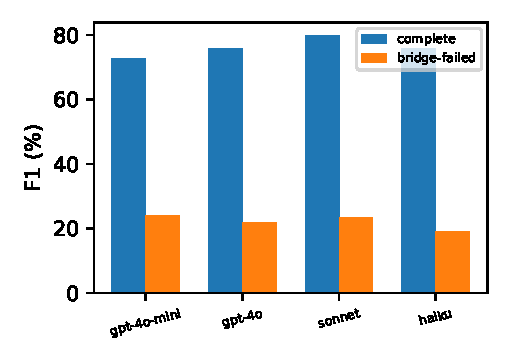
\includegraphics[width=\columnwidth]{figs/fig_link}
\caption{F1 by generator when the context is complete or bridge-failed (primary set, eight systems pooled).}
\label{fig:link}
\end{figure}

\subsection{Is spectral connectivity the active ingredient? (RQ3)}
Table~\ref{tab:abl} replaces the $\lambda_2$ term by alternatives, keeping the weight $\mu$ tuned for the normalised $\lambda_2$. The unnormalised $\lambda_2$ has a different scale, so its best $\mu$ differs; we treat the comparison as indicative. Removing the term altogether ($\mu{=}0$) costs 4.4 gold-complete points, confirming that rewarding connectivity helps. But the \emph{number of connected components} (a count, no eigenvalues) and the \emph{unnormalised} $\lambda_2$ score 2.2 and 2.8 points higher gold-complete (uncorrected intervals above zero; Holm-corrected over the eight ablation comparisons $p=0.11$, so not significant), with F1 differences within noise, and a plain density term is equivalent. Only the removal of the term ($\mu{=}0$) is significantly worse (Holm $p=0.002$ for gold-complete). The comparison is indicative: the component-count objective is integer-valued, so a common $\mu$ is not on a common scale. Sensitivity to $\mu$ (Fig.~\ref{fig:mu}) shows the same picture: the unnormalised variant peaks at 68.6\% at $\mu{=}1$, whereas the normalised variant peaks at 63.1\% at $\mu{=}0.25$. This sweep was run on the primary set after the protocol was fixed; its maximum over seven values of $\mu$ is optimistic, and it is exploratory. We conclude that the benefit comes from a connectivity reward in general, and that spectral quantities offer no demonstrated advantage over simpler ones here.

\begin{table}[t]
\centering
\caption{Ablations of the selection objective (primary set, gpt-4o-mini). $\Delta$ = variant minus SES-RAG, 95\% CI.}
\label{tab:abl}
\small
\resizebox{\columnwidth}{!}{%
\begin{tabular}{lcccc}
\toprule
Variant & Gold-complete & $\Delta$ & F1 & $\Delta$ \\
\midrule
SES-RAG (norm.\ $\lambda_2$) & 63.1 & -- & 54.8 & -- \\
Hybrid+Expand ($\mu{=}0$) & 58.7 & -4.4 [-7.1,-1.9] & 53.0 & -1.8 [-4.1,+0.4] \\
SES, component count & 65.3 & +2.2 [+0.5,+3.9] & 55.8 & +1.0 [-0.6,+2.7] \\
SES, density term & 62.5 & -0.6 [-3.1,+1.9] & 53.9 & -0.9 [-3.1,+1.2] \\
SES, raw $\lambda_2$ & 65.9 & +2.8 [+0.7,+5.0] & 55.4 & +0.6 [-1.3,+2.4] \\
\bottomrule
\end{tabular}}
\end{table}

\begin{figure}[t]
\centering
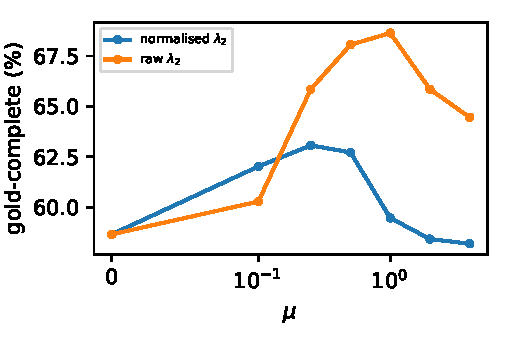
\includegraphics[width=\columnwidth]{figs/fig_mu}
\caption{Gold-complete rate of SES-RAG versus $\mu$ for the normalised and unnormalised $\lambda_2$ (primary set, exploratory sensitivity analysis).}
\label{fig:mu}
\end{figure}

\subsection{Token budget}
Figure~\ref{fig:budget} shows gold-complete retrieval for budgets from 300 to 1{,}500 tokens. SES-RAG has the highest point estimate among LLM-free methods at every budget (no intervals were computed for this sweep, and $\mu$ was not re-tuned per budget), with the largest margins at tight budgets (47.3\% at 300 tokens versus 41.0\% for the next best, GraphRAG-lite), and the curves converge as the budget grows (80.7\% vs.\ 79.9\% for SpectRAG-lite at 1{,}500, where the iterative baseline's context uses only about 1{,}000 of the 1{,}500 tokens). Connectivity-aware packing matters most when the budget forces a choice among candidates.

\begin{figure}[t]
\centering
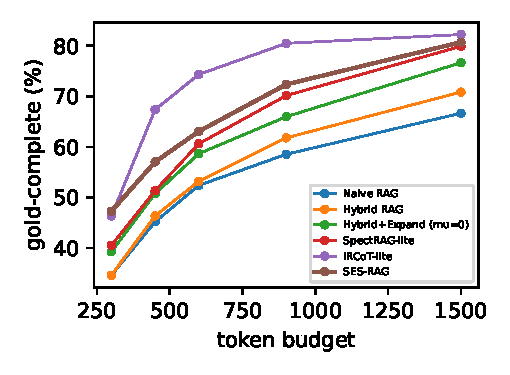
\includegraphics[width=\columnwidth]{figs/fig_budget}
\caption{Gold-complete rate versus token budget (primary set).}
\label{fig:budget}
\end{figure}

\subsection{Extension: iterative retrieval with connectivity-aware packing}
IRCoT+SES adds the iterative-retrieval candidates to the SES pool and packs the budget with the same rule (Section~\ref{sec:method}). On the development and exploration questions it improved gold-complete retrieval from 74.0\% to 77.0\%, but on the primary set it did not: 75.0\% vs.\ 74.3\% gold-complete (+0.7 points, 95\% CI $-2.0$ to $+3.4$) and 61.6\% vs.\ 61.9\% F1 ($-0.3$, CI $-2.6$ to $+2.0$). It is better than SES-RAG alone (+12.0 gold-complete, +6.8 F1 points), so the retrieval of the bridge, not the packing, accounts for IRCoT's advantage. On MuSiQue IRCoT+SES is \emph{worse} than IRCoT-lite in gold-complete rate ($-4.4$ points, 95\% CI $-7.2$ to $-1.6$) and not better on 2WikiMultiHopQA ($-0.4$, CI $-4.0$ to $+3.4$).

\subsection{Where SES-RAG loses}
The candidate pool contains every gold paragraph for 90.8\% of the primary questions, and at least one gold paragraph is a retrieval seed for 99.1\%. SES-RAG's context is complete for 63.1\%: about 28 points are lost at selection (the gold paragraphs were in the pool but not chosen) and about 9 points because the pool lacked one. Since the pool has 100 candidates for about five context slots, pool recall is a loose ceiling. In 73.3\% of questions the two gold paragraphs are directly linked in the graph.

\subsection{Dependence on the graph and transfer (RQ4)}
\paragraph{Without title-mention edges.}
We rebuilt the graph with the mention signal removed and re-tuned the parametrised systems on the development and exploration questions. Table~\ref{tab:nomention} gives gold-complete rates on the primary set. SES-RAG falls from 63.1\% to 57.5\%, no better than the $\mu{=}0$ control (58.3\%; difference $-0.8$ points, 95\% CI $-3.4$ to $+1.7$) or G-Retriever-lite (58.4\%). On this graph the re-tuned mixing weight of SpectRAG-lite is zero, which makes its selections identical to the control's, so it is not an independent comparison. GraphRAG-lite and IRCoT-lite do not read the graph and are unchanged. SES-RAG still exceeds Hybrid and Naive RAG by 4.3 and 5.1 points because the pool is expanded through the remaining entity and similarity edges; it is the connectivity reward on top of the expanded pool that no longer helps. We did not test an interaction between the graph and the reward statistically, and the spectral coordinates of SpectRAG-lite in this run use the largest connected component only. With gpt-4o-mini, SES-RAG reaches 51.5\% F1 against 52.6\% for the control and SpectRAG-lite on the same questions. The connectivity reward needs a graph that actually links bridge passages.

\begin{table}[t]
\centering
\caption{Primary set with and without title-mention edges in the graph: gold-complete rate (\%) and, where answered with gpt-4o-mini, F1 (\%).}
\label{tab:nomention}
\small
\resizebox{\columnwidth}{!}{%
\begin{tabular}{lccc}
\toprule
System & Gold-complete, with & Gold-complete, without & F1, without \\
\midrule
Naive RAG & 52.4 & 52.4 & -- \\
Hybrid RAG & 53.2 & 53.2 & -- \\
Hybrid+Expand ($\mu{=}0$) & 58.7 & 58.3 & 52.6 \\
GraphRAG-lite & 60.2 & 60.2 & -- \\
SpectRAG-lite & 60.6 & 58.3 & 52.6 \\
G-Retriever-lite & 58.9 & 58.4 & -- \\
IRCoT-lite & 74.3 & 74.3 & -- \\
SES-RAG & 63.1 & 57.5 & 51.5 \\
\bottomrule
\end{tabular}}
\end{table}

\paragraph{2WikiMultiHopQA.}
On 500 compositional and inference questions, with every setting frozen on HotpotQA and no re-tuning, SES-RAG's gold-complete rate is 43.2\%, against 23.8\% for Hybrid RAG and 33.8--34.8\% for SpectRAG-lite and GraphRAG-lite (Table~\ref{tab:2wiki}). The gold-complete gains over every LLM-free baseline (+8.4 to +19.4 points) are significant after Holm correction. F1 improves by 1.8 to 5.8 points, significantly for all but GraphRAG-lite. IRCoT-lite reaches 65.6\% gold-complete and 27.2\% F1 (SES-RAG: 21.0\%), against a ceiling of 32.6\% F1 for the gold-first oracle. The corpus here is small (5{,}173 paragraphs, many shared across questions), so absolute completeness is not comparable with HotpotQA's. At 600 tokens even the oracle fits all gold paragraphs for only 84.4\% of these questions.

\begin{table}[t]
\centering
\caption{2WikiMultiHopQA ($n=500$ questions, settings frozen on HotpotQA), gpt-4o-mini.}
\label{tab:2wiki}
\small
\resizebox{\columnwidth}{!}{%
\begin{tabular}{lcccc}
\toprule
System & Gold-complete (\%) & F1 (\%) & Judged acc. (\%) & LLM calls \\
\midrule
Naive RAG & 26.8\,{\scriptsize[22.8,30.8]} & 16.0\,{\scriptsize[13.1,18.9]} & 15.4\,{\scriptsize[12.2,18.6]} & 0 \\
Hybrid RAG & 23.8\,{\scriptsize[20.2,27.4]} & 15.1\,{\scriptsize[12.4,18.0]} & 14.2\,{\scriptsize[11.2,17.2]} & 0 \\
Hybrid+Expand ($\mu{=}0$) & 29.2\,{\scriptsize[25.2,33.2]} & 16.8\,{\scriptsize[14.0,19.7]} & 16.8\,{\scriptsize[13.6,20.2]} & 0 \\
GraphRAG-lite & 34.8\,{\scriptsize[30.6,39.2]} & 19.1\,{\scriptsize[16.0,22.4]} & 20.0\,{\scriptsize[16.6,23.6]} & 0 \\
SpectRAG-lite & 33.8\,{\scriptsize[29.6,38.0]} & 18.4\,{\scriptsize[15.4,21.6]} & 18.2\,{\scriptsize[15.0,21.6]} & 0 \\
G-Retriever-lite & 30.4\,{\scriptsize[26.4,34.6]} & 17.0\,{\scriptsize[14.0,20.0]} & 16.8\,{\scriptsize[13.6,20.2]} & 0 \\
IRCoT-lite & 65.6\,{\scriptsize[61.6,69.8]} & 27.2\,{\scriptsize[23.6,30.6]} & 28.4\,{\scriptsize[24.4,32.2]} & 3 \\
\textbf{SES-RAG} & 43.2\,{\scriptsize[38.8,47.6]} & 21.0\,{\scriptsize[17.8,24.1]} & 21.2\,{\scriptsize[17.6,24.8]} & 0 \\
IRCoT+SES & 65.2\,{\scriptsize[61.0,69.4]} & 27.2\,{\scriptsize[23.5,30.7]} & 28.6\,{\scriptsize[24.6,32.4]} & 3 \\
\midrule
Gold-first oracle & 84.4\,{\scriptsize[81.2,87.6]} & 32.6\,{\scriptsize[28.9,36.2]} & 34.2\,{\scriptsize[30.0,38.0]} & -- \\
\bottomrule
\end{tabular}}
\end{table}

Table~\ref{tab:transfer_tests} lists the paired comparisons for both external datasets.

\paragraph{MuSiQue.}
MuSiQue questions need two to four hops and every method struggles (Table~\ref{tab:musique}): gold-complete rates are 16--22\% for all LLM-free systems and SES-RAG (21.4\%) is indistinguishable from the control, Naive RAG, GraphRAG-lite, SpectRAG-lite and G-Retriever-lite; it improves only on Hybrid RAG (+5.0 points, Holm $p=0.003$). IRCoT-lite is 10 points ahead (31.8\%). The connectivity reward therefore does not transfer to these deeper chains at this budget.

\begin{table}[t]
\centering
\caption{MuSiQue ($n=500$ questions, settings frozen on HotpotQA), gpt-4o-mini.}
\label{tab:musique}
\small
\resizebox{\columnwidth}{!}{%
\begin{tabular}{lcccc}
\toprule
System & Gold-complete (\%) & F1 (\%) & Judged acc. (\%) & LLM calls \\
\midrule
Naive RAG & 21.2\,{\scriptsize[17.6,24.8]} & 16.3\,{\scriptsize[13.3,19.5]} & 18.2\,{\scriptsize[14.8,21.6]} & 0 \\
Hybrid RAG & 16.4\,{\scriptsize[13.2,19.8]} & 13.3\,{\scriptsize[10.7,16.1]} & 14.4\,{\scriptsize[11.4,17.6]} & 0 \\
Hybrid+Expand ($\mu{=}0$) & 21.4\,{\scriptsize[18.0,25.0]} & 16.9\,{\scriptsize[14.0,20.1]} & 18.4\,{\scriptsize[15.0,22.0]} & 0 \\
GraphRAG-lite & 20.8\,{\scriptsize[17.4,24.4]} & 16.8\,{\scriptsize[13.9,20.1]} & 17.8\,{\scriptsize[14.6,21.2]} & 0 \\
SpectRAG-lite & 21.0\,{\scriptsize[17.4,24.6]} & 15.8\,{\scriptsize[13.0,18.8]} & 17.4\,{\scriptsize[14.2,20.8]} & 0 \\
G-Retriever-lite & 21.8\,{\scriptsize[18.2,25.4]} & 15.9\,{\scriptsize[13.1,19.0]} & 17.6\,{\scriptsize[14.4,20.8]} & 0 \\
IRCoT-lite & 31.8\,{\scriptsize[27.6,35.8]} & 24.2\,{\scriptsize[20.8,27.8]} & 25.6\,{\scriptsize[22.0,29.6]} & 3 \\
\textbf{SES-RAG} & 21.4\,{\scriptsize[17.8,25.0]} & 16.6\,{\scriptsize[13.6,19.6]} & 18.0\,{\scriptsize[14.6,21.4]} & 0 \\
IRCoT+SES & 27.4\,{\scriptsize[23.4,31.2]} & 22.2\,{\scriptsize[18.9,25.7]} & 24.2\,{\scriptsize[20.4,28.2]} & 3 \\
\midrule
Gold-first oracle & 92.4\,{\scriptsize[90.2,94.8]} & 32.8\,{\scriptsize[29.2,36.7]} & 34.6\,{\scriptsize[30.6,38.6]} & -- \\
\bottomrule
\end{tabular}}
\end{table}
\begin{table}[t]
\centering
\caption{SES-RAG minus each baseline on the external datasets (gpt-4o-mini; $\Delta$ in points, 95\% CI, Holm $p$ over the 14 comparisons per dataset).}
\label{tab:transfer_tests}
\small
\resizebox{\columnwidth}{!}{%
\begin{tabular}{llllcc}
\toprule
Dataset & Baseline & Metric & $\Delta$ & 95\% CI & Holm $p$ \\
\midrule
MuSiQue & Naive RAG & Gold-complete & +0.2 & [-2.8, +3.0] & 1.000 \\
MuSiQue & Naive RAG & F1 & +0.2 & [-2.2, +2.6] & 1.000 \\
MuSiQue & Hybrid RAG & Gold-complete & +5.0 & [+2.4, +7.8] & 0.003 \\
MuSiQue & Hybrid RAG & F1 & +3.2 & [+0.6, +5.8] & 0.094 \\
MuSiQue & Hybrid+Expand ($\mu{=}0$) & Gold-complete & +0.0 & [-2.2, +2.2] & 1.000 \\
MuSiQue & Hybrid+Expand ($\mu{=}0$) & F1 & -0.4 & [-2.5, +1.7] & 1.000 \\
MuSiQue & GraphRAG-lite & Gold-complete & +0.6 & [-2.0, +3.2] & 1.000 \\
MuSiQue & GraphRAG-lite & F1 & -0.3 & [-2.6, +2.0] & 1.000 \\
MuSiQue & SpectRAG-lite & Gold-complete & +0.4 & [-2.0, +2.8] & 1.000 \\
MuSiQue & SpectRAG-lite & F1 & +0.7 & [-1.7, +3.1] & 1.000 \\
MuSiQue & G-Retriever-lite & Gold-complete & -0.4 & [-2.8, +2.0] & 1.000 \\
MuSiQue & G-Retriever-lite & F1 & +0.6 & [-1.4, +2.7] & 1.000 \\
MuSiQue & IRCoT-lite & Gold-complete & -10.4 & [-14.2, -6.8] & 1.000 \\
MuSiQue & IRCoT-lite & F1 & -7.7 & [-10.9, -4.5] & 1.000 \\
2Wiki & Naive RAG & Gold-complete & +16.4 & [+12.8, +20.0] & $<$0.001 \\
2Wiki & Naive RAG & F1 & +5.0 & [+2.8, +7.4] & $<$0.001 \\
2Wiki & Hybrid RAG & Gold-complete & +19.4 & [+15.8, +23.2] & $<$0.001 \\
2Wiki & Hybrid RAG & F1 & +5.8 & [+3.4, +8.4] & $<$0.001 \\
2Wiki & Hybrid+Expand ($\mu{=}0$) & Gold-complete & +14.0 & [+10.8, +17.2] & $<$0.001 \\
2Wiki & Hybrid+Expand ($\mu{=}0$) & F1 & +4.1 & [+2.1, +6.3] & 0.001 \\
2Wiki & GraphRAG-lite & Gold-complete & +8.4 & [+5.0, +12.0] & $<$0.001 \\
2Wiki & GraphRAG-lite & F1 & +1.8 & [-0.7, +4.3] & 0.201 \\
2Wiki & SpectRAG-lite & Gold-complete & +9.4 & [+6.2, +12.8] & $<$0.001 \\
2Wiki & SpectRAG-lite & F1 & +2.5 & [+0.3, +4.8] & 0.043 \\
2Wiki & G-Retriever-lite & Gold-complete & +12.8 & [+9.6, +16.2] & $<$0.001 \\
2Wiki & G-Retriever-lite & F1 & +4.0 & [+1.7, +6.2] & 0.001 \\
2Wiki & IRCoT-lite & Gold-complete & -22.4 & [-27.2, -17.4] & 1.000 \\
2Wiki & IRCoT-lite & F1 & -6.2 & [-9.6, -2.9] & 1.000 \\
\bottomrule
\end{tabular}}
\end{table}
\begin{table}[t]
\centering
\caption{External datasets by generator: gold-complete (\%) is generator-independent; F1 (\%) differs by generator.}
\label{tab:extgen}
\small
\resizebox{\columnwidth}{!}{%
\resizebox{\columnwidth}{!}{%
\begin{tabular}{llccccc}
\toprule
Dataset & Generator & Naive & SpectRAG-lite & IRCoT-lite & SES-RAG & Oracle \\
\midrule
MuSiQue & gpt-4o-mini & 21.2 / 16.3 & 21.0 / 15.8 & 31.8 / 24.2 & 21.4 / 16.6 & 92.4 / 32.8 \\
MuSiQue & claude-sonnet-5-5 & 21.2 / 20.4 & 21.0 / 20.2 & 31.8 / 30.1 & 21.4 / 19.8 & 92.4 / 47.6 \\
2Wiki & gpt-4o-mini & 26.8 / 16.0 & 33.8 / 18.4 & 65.6 / 27.2 & 43.2 / 21.0 & 84.4 / 32.6 \\
2Wiki & claude-sonnet-5-5 & 26.8 / 20.4 & 33.8 / 23.1 & 65.6 / 40.2 & 43.2 / 29.3 & 84.4 / 50.4 \\
\bottomrule
\end{tabular}}}
\end{table}

Table~\ref{tab:extgen} repeats the comparison with claude-sonnet-5-5 as generator. The ordering of SES-RAG, SpectRAG-lite and IRCoT-lite is unchanged, and on 2WikiMultiHopQA absolute F1 is higher for Claude (IRCoT-lite 40.2\%, oracle 50.4\%) than for gpt-4o-mini (27.2\%, 32.6\%), so the oracle abstention ceiling noted below is generator-specific.

\paragraph{A caveat on answer metrics for the external datasets.} Even when the gold paragraphs are the whole context, gpt-4o-mini abstains on 48\% of 2WikiMultiHopQA and 48\% of MuSiQue questions (9.6\% on HotpotQA), so the labelled supporting paragraphs are often not enough for the model to commit to an answer. F1 on these datasets is therefore capped well below HotpotQA's (oracle F1: 32.6\% and 32.8\%), and we regard the gold-complete rate as the more reliable metric there. Hybrid RAG is also below Naive RAG on both external datasets, so fusion with BM25 is not uniformly helpful in this setting.


\subsection{Cost}
Selecting the context with SES-RAG takes 3.7\,ms per question on a CPU, given the shared candidate pool, and requires no LLM call; the corresponding selection step takes 0.03\,ms for Hybrid RAG and 0.2\,ms for SpectRAG-lite. The timings exclude pool construction, BM25 scoring and graph building, which all graph-based systems share. IRCoT-lite needs three sequential LLM calls (plus three embedding calls) per question before the answer is generated.

\section{Discussion}
\label{sec:discussion}

\paragraph{What the evidence supports.}
Bridge failure is the dominant source of loss on bridge questions: for every generator, answer F1 collapses and abstention rises sharply when the context lacks a gold paragraph (Table~\ref{tab:link}). Closing the retrieval gap is therefore worth a large amount of answer quality, up to the 71--79\% F1 of the gold-first oracle. Among methods that make no LLM call, SES-RAG has the highest gold-complete rate at all five budgets we tested (300 to 1{,}500 tokens), by a margin that shrinks to under one point at 1{,}500 tokens (Fig.~\ref{fig:budget}); at 300 tokens it is nominally ahead of the iterative baseline as well (47.3\% vs.\ 46.3\%, not tested). Its F1 advantage over Hybrid RAG is stable across four generators. Its F1 lead over GraphRAG-lite and SpectRAG-lite is 1.2 to 3.7 points; the uncorrected intervals exclude zero for three of four generators against GraphRAG-lite and two of four against SpectRAG-lite, but not under the Holm correction used for the primary generator.

\paragraph{What it does not support.}
Three claims that one might expect from a spectral formulation are not supported. (i) SES-RAG is not significantly better than the strongest graph baselines (GraphRAG-lite, SpectRAG-lite) after Holm correction. (ii) $\lambda_2$ is not the active ingredient: replacing it by the number of connected components (a simpler quantity) or by an unnormalised $\lambda_2$ matches or exceeds it (Table~\ref{tab:abl}), so what matters is rewarding a \emph{connected} context, not the particular spectral measure. The structure of the normalised $\lambda_2$ offers a likely explanation: it falls as a connected set grows, so the reward mostly penalises fragmentation and gives no credit for extending a chain (Section~\ref{sec:method}); a component count measures fragmentation directly and is unaffected by growth. (iii) An LLM-driven iterative retriever is clearly ahead, by 11 points of gold-complete rate and 7--10 points of F1 depending on the generator, at the price of three LLM calls per question.

\paragraph{Where the loss occurs.}
The candidate pool contains all gold paragraphs for 90.8\% of questions, yet SES-RAG's context is gold-complete for 63.1\%. Pool recall is a loose ceiling, since the pool holds 100 candidates for about five context slots, but it shows that the relevance score and the connectivity reward often fail to single out the bridge among many candidates. The iterative retriever, which finds the bridge with LLM-written queries, is 11 points ahead, and packing its candidates with our rule does not help. Connectivity alone does not discriminate: in 26.7\% of questions the two gold paragraphs have no direct graph edge, and distractors connected to the seeds compete for the same budget.

\paragraph{Dependence on the graph.}
The signal that makes connectivity informative is the title-mention edge, which mirrors hyperlinks between encyclopedia articles. Without it, the advantage of SES-RAG over the graph baselines vanishes (Table~\ref{tab:nomention}). This is consistent with the idea that a connectivity reward can only help if the graph encodes the bridge relation; we did not test this with other kinds of links. The mention edges mirror the hyperlink structure that defines HotpotQA's bridges, so the result is also a statement about how favourable the benchmark graph is. Corpora without explicit links would need link prediction, entity linking or an LLM-built graph.

\paragraph{Practical guidance.}
When query-time LLM calls are acceptable, iterative retrieval is the stronger choice. When latency or cost forbids them, a connectivity-aware selector over a link-aware graph is the best option we evaluated, and selection takes about four milliseconds per question on a CPU. Combining the two (IRCoT+SES) did not help on the primary set and lowered gold-complete retrieval on MuSiQue, which suggests that the benefit of connectivity-aware packing is small once the retriever already finds the bridge.

\section{Limitations}
\label{sec:limits}
\begin{itemize}
\item \textbf{Simplified baselines.} GraphRAG-lite, SpectRAG-lite, G-Retriever-lite and IRCoT-lite re-implement the retrieval principle of each system on one shared graph; they omit LLM-built graphs, community summaries, learned components and, for IRCoT, chain-of-thought reasoning inside the loop. Conclusions about the original systems cannot be drawn from them.
\item \textbf{Graph construction.} Title-mention edges rely on encyclopedic titles. The corpus pools 2{,}000 questions' paragraphs, which is much smaller than a full Wikipedia index.
\item \textbf{Evaluation.} The primary dataset is HotpotQA bridge questions; the external datasets use settings frozen on HotpotQA. Against a second judge (gpt-4o, 10\% random subsample per generator) the correctness judgments agree 91.6--93.4\% ($\kappa=0.62$--$0.75$), but the faithfulness judgments only 83.6--88.3\% ($\kappa=0.18$--$0.53$), so we do not base any claim on faithfulness or the unsupported-answer rate. Both judges are LLMs and no human validation was done; claude-haiku-5-5 judges its own answers as well as those of the other generators.
\item \textbf{Generators.} Four generators from two vendors were used; the Claude models accept no temperature parameter and ran with default sampling, so their results are not strictly deterministic. A third vendor could not be evaluated at scale because of API quota limits.
\item \textbf{Scope.} Comparison questions, which need parallel rather than chained evidence, are outside the study. In an earlier mixed-type run (different generator and protocol, so only indicative) SES-RAG retrieved a gold-complete context for 59\% of comparison questions against 89--95\% for the baselines, because the connectivity reward pulls the selection towards a chain.
\item \textbf{External-dataset answer metrics.} On 2WikiMultiHopQA and MuSiQue the gold-first oracle abstains on about 48\% of questions, so F1 is capped far below HotpotQA's and we rely on the gold-complete rate there.
\item \textbf{Answer format and judging.} The Claude generators produce answers of 60 or more characters for about 8\% of questions against under 1\% for the OpenAI models, so F1 and judged accuracy are not format-controlled across vendors, and Sonnet and Haiku were run with different thinking settings (necessarily, as the API requires different values). The judge's accuracy exceeds the F1-threshold accuracy by 2.5 points for both Claude generators and by 0.9 and 1.6 points for gpt-4o-mini and gpt-4o.
\item \textbf{Statistics.} One generation run per generator and system; no human validation of the judge; ablation intervals are not corrected beyond the primary family; the $\mu$ and budget sweeps were run on the primary set and are exploratory.
\item \textbf{Artifacts.} The code and outputs are in the project repository; a public repository URL and archival DOI are to be added at submission.
\end{itemize}


\section{Conclusion}
\label{sec:conclusion}
Bridge failure, a context that holds the endpoints of a reasoning chain but not the passage linking them, is strongly associated with the answer-quality loss on bridge questions for every generator we tested (F1 drops by 48--57 points between complete and failed contexts, also within the same question). A connectivity-aware selector that uses no LLM call recovers part of that loss: on HotpotQA it gives about 10 more points of gold-complete retrieval and 4.0--6.5 more F1 points than Hybrid RAG, and on 2WikiMultiHopQA it leads all LLM-free baselines by 8--19 points of gold-complete retrieval. The study also delimits the claim. The spectral form of the connectivity reward is not necessary, the benefit requires a graph that links bridge passages, it does not transfer to MuSiQue's deeper chains, and iterative LLM retrieval remains clearly stronger when its cost is acceptable. The iterative retriever, which finds the bridge passage with LLM-written queries, shows that candidate generation remains the larger lever; a connectivity-aware selector cannot recover a bridge that the relevance score and graph never surface. Better bridge discovery without per-query LLM calls, learned or LLM-assisted selection over a connected candidate pool, and graph construction for corpora without explicit links are the natural next steps.


\section*{Availability}
Code, frozen parameters, cached model outputs and all result tables are in the project repository (\texttt{experiment/results/}); every number in this paper is generated from those files.

\bibliographystyle{IEEEtran}
\bibliography{refs}
\end{document}
